\documentclass[conference]{IEEEtran}
%+++++++++++++++++++++++++++++++++++++++++++
% Added to commands
\input epsf
\usepackage{graphicx}
\usepackage [french]{babel}
\usepackage [utf8]{inputenc}
\usepackage [T1] {fontenc}
\usepackage{float}
%+++++++++++++++++++++++++++++++++++++++++++
% correct bad hyphenation here
\hyphenation{op-tical net-works semi-conduc-tor IEEEtran}
\begin{document}

%+++++++++++++++++++++++++++++++++++++++++++
\title{\LARGE Mesure de l'angle du kite au Zentith 
\vskip10pt

\small 2024 - Romain LAMBERT
}
%+++++++++++++++++++++++++++++++++++++++++++
% make the title area
\maketitle

\begin{abstract}Ce bureau d'étude a pour sujet l'équilibre au Zénith du Kite. L'objectif final étant de déterminer un protocol expérimental permetant de mesurer l'angle d'incidence d'un kite; en vue d'obtenir une polaire expérimentale des voiles. 
\end{abstract}
\IEEEoverridecommandlockouts

\IEEEpeerreviewmaketitle
\section{Travaux précédents (Zoé Marcelet)}

\subsection{Modèle Lagragien} 

D'après le document \textit{"Dynamics and Control of Single-Line Kites"} de Gonzalo Sanchez-Arriaga (2006),  les formules suivantes permettent d'obtenir l'élévation $\Gamma$ et l'angle d'incidence du vent $\theta$, en fonction du vent et des coefficients aérodynamiques du kite : \\

\begin{figure}[H]
    \centering
    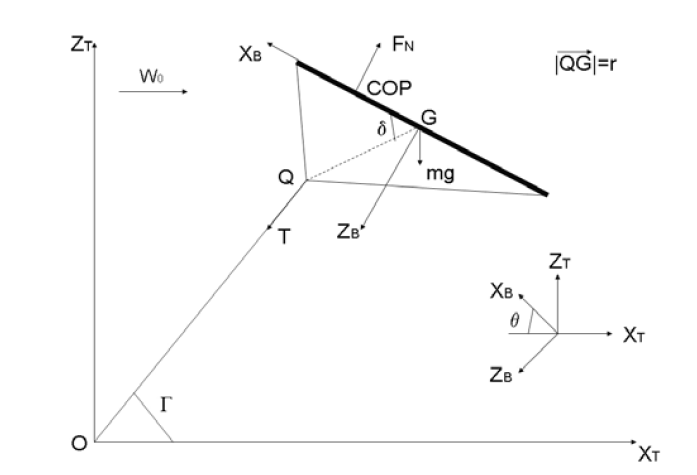
\includegraphics[width=0.5\textwidth]{Pics/Picture Sanchez.png}  
    \caption{Schéma du kite au Zénith.}
    \label{fig:sanchez}
\end{figure}

La première équation donne l’angle d’incidence $\theta$ : 
\begin{center}
    \begin{equation}
        cos(\delta - \theta) + \beta (\sigma-cos(\delta))C_N(\theta) = 0
        \label{eq:theta}
    \end{equation}
\end{center}
La deuxieme équation donne l’angle d’élévation $\Gamma$ :
\begin{center}
    \begin{equation}
        \Gamma = tan^{-1}(\frac{\beta C_N (\theta) cos(\theta)-1}{\beta C_N (\theta)sin(\theta)})
        \label{eq:gamma}
    \end{equation}
\end{center}
Avec $\beta = \frac{\rho A W_0^2}{2mg}$ et $\sigma = \frac{X_{cp}}{r}$ \\

Ces équations ont été codées (disponible sur Nextcloud : 06-RESSOURCE/AC-Admin Commun/4-Rapports Stagiaires/Stage Zoé Marcelet/Rapport\_zozo/06\_Topic\_modèle\_aéro\_zenith). 
Elles restent cependant peut concluantes car requièrent les coéfficients aérodynamiques du kite. 

\IEEEpeerreviewmaketitle
\section{Mesure de l'angle d'incidence au Zénith}

\subsection{Problème de l'angle de calage $\alpha_0$} 


Une première intuition nous amène à penser que la connaissance de l'angle d'élévation et de la géométrie des bridages permet de remonter à l'angle d'incidence $\alpha$

\begin{figure}[H]
    \centering
    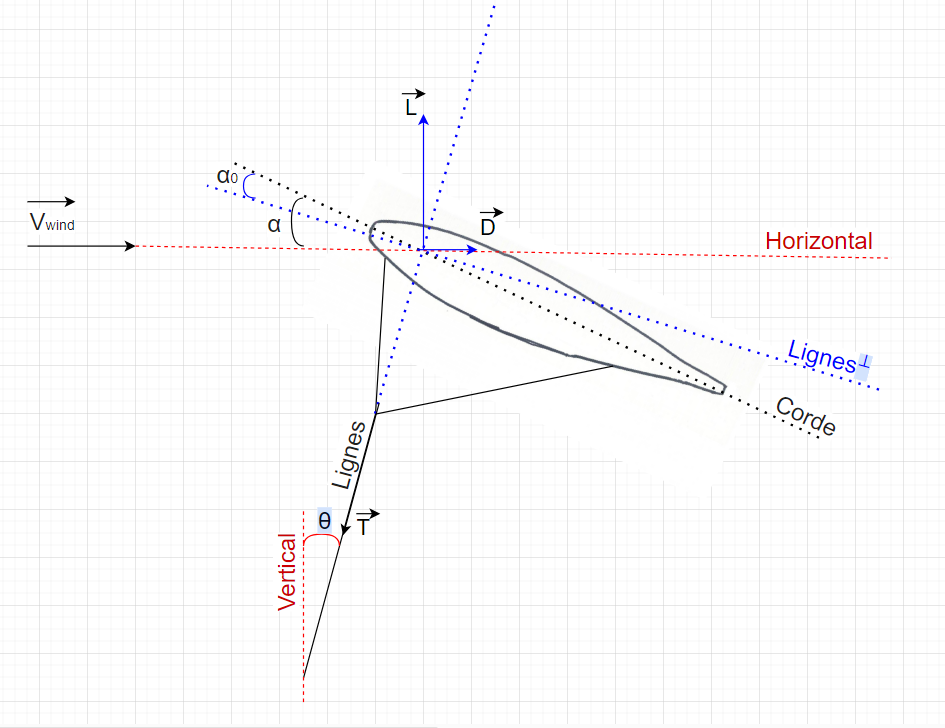
\includegraphics[width=0.5\textwidth]{Pics/Schéma Equilibre Zéntih.png}  
    \caption{Schéma des angles qui paramètres le Zénith.}
    \label{fig:Zénith alpha zéro}
\end{figure}

La figure \ref{fig:Zénith alpha zéro}, l'angle $\alpha_0$ dépend de considération aérodynamique, car : 
\begin{center}
    \begin{equation}
        \frac{L}{D} = \frac{1}{tan(\theta)} = \frac{1}{tan(\alpha + \alpha_0)}
    \end{equation}
\end{center}
Ainsi, l'angle que fait le cône de bridage avec les lignes qui le relient au sol s'adapte (via l'angle $\alpha_0$) de sorte à aligner les efforts aérodynamiques avec les lignes des avants. Ainsi, cette angle permet de lier "géométrie" et "aérodynamique" :  

\begin{figure}[H]
    \centering
    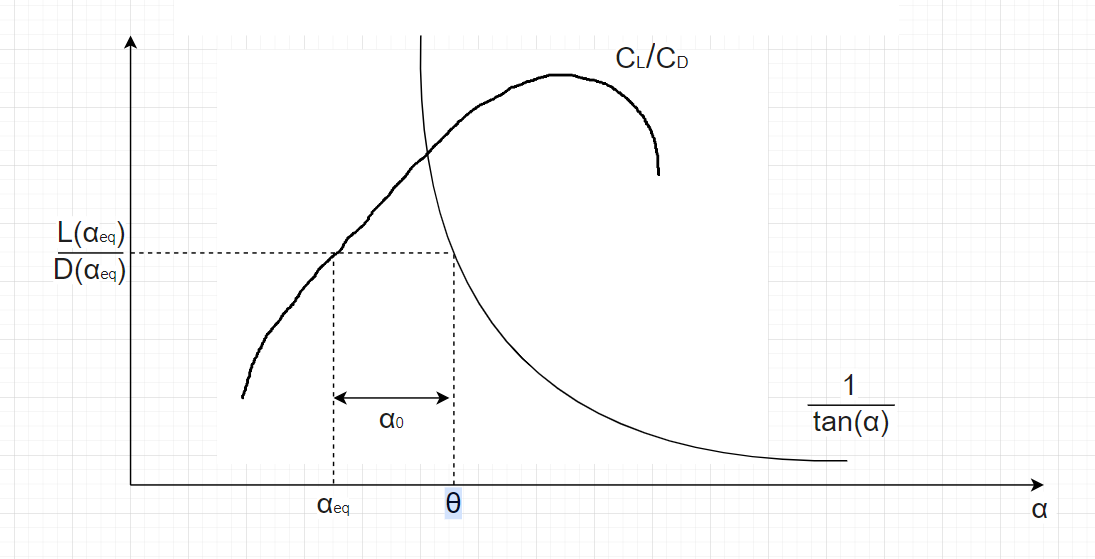
\includegraphics[width=0.5\textwidth]{Pics/Schéma Equilibre finesse.png}  
    \caption{Graphique du lien entre finesse (aérodynamique) et l'angle $\alpha_0$}
    \label{fig:Zénith finesse}
\end{figure}

\textbf{Cependant,} la formule à l'équilibre suivante (voir "equilibre kite" pour demo) : 

\begin{center}
    \begin{equation}
        x_T = \frac{L x_F - P x_G -C_{M_0}}{L - P}
    \end{equation}
\end{center}

montre qu'en \textbf{vent fort}, pour $C_{M_0} = 0$, $x_T = x_F$, et donc on peut déterminer géométriquement $\alpha_0$ ! \textbf{Donc la mesure de l'angle $\theta$ permet de remonter à $\alpha$ et la finesse $\frac{L}{D}$}

\subsection{Utiliser un capteur de tension pour les A et les B au niveau du kite}

L'idée est que notre système \{kite+bridages\} se comporte comme un pendule inversé. Mesurer les tensions dans les A et les B permet de mesurer la position de la résultante aérodynamique le long du kite et ainsi de prédire son angle d'incidence $\alpha$ en s'affranchissant de la polaire aérodynamique du kite. 

\begin{figure}[H]
    \centering
    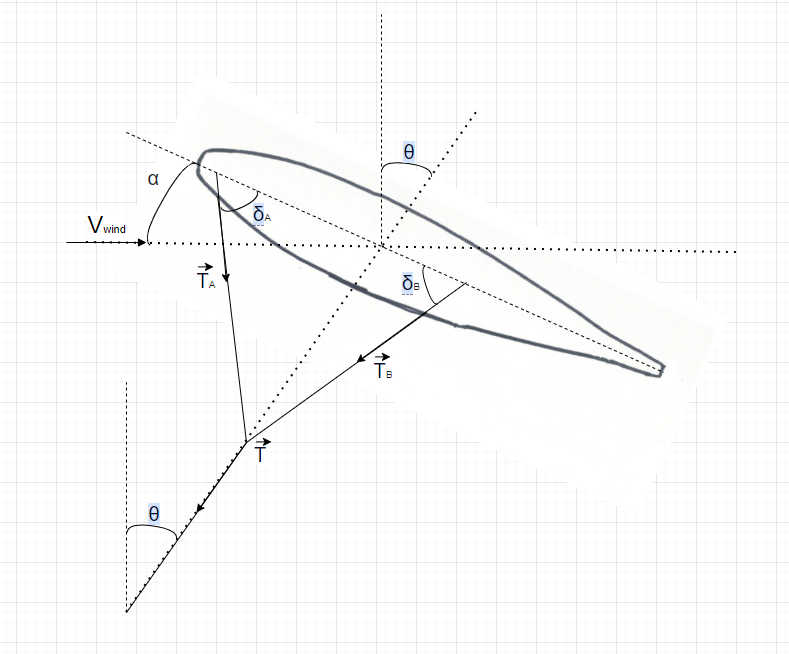
\includegraphics[width=0.5\textwidth]{Pics/Schéma Equilibre capteurs tension AB.png}  
    \caption{Schéma des tensions dans les bridages}
    \label{fig:Zénith tensions AB}
\end{figure}

Le graphe \ref{fig:Zénith tensions AB} permet d'écrire la relation suivante : 
\begin{center}
    \begin{equation}
        T_A cos(\delta_A) - T_B cos(\delta_B) = T cos(\frac{\pi}{2} +\alpha - \theta)
    \end{equation}
\end{center}

et ainsi d'en déduire :

\begin{center}
    \begin{equation}
        \alpha = \theta + sin^{-1}(\frac{T_B cos(\delta_B) - T_A cos(\delta_A)}{T}))
    \end{equation}
\end{center}

Ainsi, on peut déterminer l'angle d'incidence $\alpha$ à partir de :
\begin{itemize}
    \item T : la tension des avants ( capteur "3 axes" )
    \item $\theta$ : $\frac{\pi}{2}$ - l'angle d'élévation (capteur "IMU")
    \item $T_A$ : la tension dans les A au point d'attache du kite (capteur "cyclopes")
    \item $T_B$ : la tension dans les B au point d'attache du kite (capteur "cyclopes")
    \item $\delta_A$ : l'angle des A par rapport à la corde moyenne du kite (surfplan ou au laser)
    \item $\delta_B$ : l'angle des B par rapport à la corde moyenne du kite (surfplan ou au laser)
\end{itemize}

\end{document}